\section{\RU{Предисловие}\EN{Preface}}

\RU{Здесь (будет) немного моих заметок о \gls{reverse engineering} на русском языке для начинающих, 
для тех кто хочет научиться понимать создаваемый \CCpp компиляторами код для x86 (коего, 
практически, больше всего остального) и ARM.}
\EN{Here are some of my notes about \gls{reverse engineering} in English language for 
those beginners who would like to learn to understand x86 (which accounts for almost 
all executable software in the world) and ARM code created by \CCpp compilers.}

\RU{У термина ``\gls{reverse engineering}'' несколько популярных значений: 
1) исследование скомпилированных
программ; 2) сканирование трехмерной модели для последующего копирования;
3) восстановление структуры СУБД. Настоящий сборник заметок
связан с первым значением}
\EN{There are several popular meanings of the term ``\gls{reverse engineering}'': 
1) reverse engineering of software: researching of compiled programs;
2) 3D model scanning and reworking in order to make a copy of it;
3) recreating \ac{DBMS} structure.
These notes are related to the first meaning.}

\subsection*{\RU{Рассмотренные темы}\EN{Topics discussed}}

x86, ARM.

\subsection*{\RU{Затронутые темы}\EN{Topics touched}}

\oracle (\ref{oracle}),
Itanium (\ref{itanium}),
\RU{донглы для защиты от копирования}\EN{copy-protection dongles} (\ref{dongles}), 
LD\_PRELOAD (\ref{ld_preload}),
\RU{переполнение стека}\EN{stack overflow}, 
\ac{ELF},
\RU{формат файла PE в win32}\EN{win32 PE file format} (\ref{win32_pe}),
x86-64 (\ref{x86-64}),
\RU{критические секции}\EN{critical sections} (\ref{critical_sections}),
\RU{сисколлы}\EN{syscalls} (\ref{syscalls}), 
\ac{TLS},
\RU{адресно-независимый код}\EN{position-independent code} (\ac{PIC}) (\ref{sec:PIC}), 
profile-guided optimization (\ref{PGO}),
C++ STL (\ref{cpp_STL}),
OpenMP (\ref{openmp}),
SEH (\label{sec:SEH}).

\subsection*{\RU{Еще кое-что}\EN{Couple of things}}

\newcommand{\FNURLREDDIT}{\footnote{\url{http://www.reddit.com/r/ReverseEngineering/}}}

\EN{Why one should learn assembly language these days?}
\RU{Зачем в наше время нужно изучать язык ассемблера?}
\EN{Unless you are OS developer, you probably don't need write in assembly: 
modern compiler do optimizations much better than humans}
\RU{Если вы не разработчик OS, вам наверное не нужно писать на ассемблере:
современные компиляторы оптимизируют код намного лучше человека}
\footnote{\RU{Очень хороший текст на эту тему}\EN{Very good text about it}: \cite{AgnerFog}}.
\EN{Modern \ac{CPU}s are very complex devices as well, and assembly knowledge would 
not help one to understand its internals.}
\RU{Современные \ac{CPU} это также крайне сложные устройства, и знание ассемблера врядли
поможет узнать его внутренности.}
\EN{But there are still at least two areas where good assembly understanding may help:
1) security/malware research; 2) better understanding of your compiled code while debugging.}
\RU{Но все-таки остается по крайней мере две области, где знание ассемблера может хорошо
помочь:
1) исследование malware (\IT{зловредов}) в целях security research; 2) лучшее понимание
вашего скомпилированного кода в процессе отладки.}

\EN{Hence, this book is intended to those who wants to understand assembly language rather 
than to write in it, and that's why here a lot of examples connected to compilers output.}
\RU{Таким образом, эта книга предназначена для тех, кто хочет скорее понимать ассемблер,
нежели писать на нем, и вот почему здесь масса примеров связанных с результатами
работы компиляторов.}

\RU{Как можно найти работу reverse engineer-а}\EN{How would one search for a reverse engineering job}? \\
\RU{На reddit, посвященному RE\FNURLREDDIT, время от времени бывают hiring thread}
\EN{There are hiring threads that appear from time to time on reddit devoted to RE\FNURLREDDIT}
(\href{http://www.reddit.com/r/ReverseEngineering/comments/1hywvr/rreverseengineerings_q3_2013_hiring_thread/}{2013 Q3}, 
\href{http://www.reddit.com/r/ReverseEngineering/comments/1vui22/rreverseengineerings_2014_hiring_thread/}{2014}).
\RU{Посмотрите там}\EN{Try to take a look there}.

\subsection*{\RU{Об авторе}\EN{About the author}}

\begin{tabularx}{\textwidth}{ l X }

\raisebox{-\totalheight}{
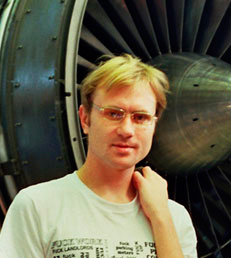
\includegraphics[scale=0.60]{Dennis_Yurichev.jpg}
}

&
\RU{Денис Юричев ~--- опытный reverse engineer и программист.
С его резюме можно ознакомиться на его сайте}
\EN{Dennis Yurichev is an experienced reverse engineer and programmer.
His CV is available on his website}\footnote{\url{http://yurichev.com/Dennis_Yurichev.pdf}}. \\
% FIXME: no link. \tablefootnote doesn't work
\end{tabularx}

\subsection*{\RU{Благодарности}\EN{Thanks}}

\RU{Тем, кто много помогал мне отвечая на массу вопросов}\EN{To those who answered all my
questions patiently}:
\HERMIT, \RU{Слава ''Avid'' Казаков}\EN{Slava ''Avid'' Kazakov}.

\RU{Тем, кто прислал много замечаний}\EN{To those who had sent me a lot of notes}:
\RU{Станислав ''Beaver'' Бобрицкий, Александр Лысенко}
\EN{Stanislav ''Beaver'' Bobrytskyy, Alexander Lysenko}, Shell Rocket.

\RU{Просто помогали разными способами}\EN{To those who just helped me in other ways}:
\RU{Андрей Зубинский}\EN{Andrew Zubinski}, 
Arnaud Patard (rtp \RU{на}\EN{on} \#debian-arm IRC).

\RU{Корректорам}\EN{To proofreaders}:
\RU{Александр ''Lstar'' Черненький}\EN{Alexander ''Lstar'' Chernenkiy},
\RU{Владимир Ботов}\EN{Vladimir Botov},
\RU{Марк}\EN{Mark} ``Logxen'' \RU{Купер}\EN{Cooper},
Yuan Jochen Kang.

\RU{И еще всем тем на github.com кто присылал замечания и коррективы}
\EN{And all the folks on github.com who have contributed notes and corrections}.

\RU{Было использовано множество пакетов \LaTeX{}: их авторов я также хотел бы поблагодарить}
\EN{A lot of \LaTeX{} packages were used: I would thank their authors as well}.

\subsection*{\RU{Отзывы об этой книге}\EN{Praise for \IT{\TITLE}}}

\begin{itemize}
\item ``It's very well done .. and for free .. amazing.''\footnote{\url{https://twitter.com/daniel_bilar/status/436578617221742593}} Daniel Bilar, Siege Technologies, LLC.

\item ``...excellent and free''\footnote{\url{https://twitter.com/petefinnigan/status/400551705797869568}} Pete Finnigan, \RU{гуру по безопасности }\oracle\EN{ security guru}.

\item ``... book is interesting, great job!'' Michael Sikorski, \RU{автор книги}\EN{author of} \IT{Practical Malware Analysis: The Hands-On Guide to Dissecting Malicious Software}.

\item ``... my compliments for the very nice tutorial!'' Herbert Bos, \RU{профессор университета}\EN{full professor at the} Vrije Universiteit Amsterdam.

\item ``... It is amazing and unbelievable.'' Luis Rocha, CISSP / ISSAP, Technical Manager, Network \& Information Security at Verizon Business.

\item ``Thanks for the great work and your book.'' Joris van de Vis, SAP Netweaver \& Security specialist.

\item ``... reasonable intro to some of the techniques.''\footnote{\url{http://www.reddit.com/r/IAmA/comments/24nb6f/i_was_a_professional_password_cracker_who_taught/}} (Mike Stay, teacher at the Federal Law Enforcement Training Center, Georgia, US.)

\end{itemize}

\subsection{\RU{Пожертвования}\EN{Donate}}
\label{sec:donate}

\RU{Как выясняется, быть (техническим) писателем требует много сил и работы}
\EN{As it turns out, (technical) writing takes a lot of effort and work}.

\RU{Эта книга является свободной, находится в свободном доступе, и доступна в виде исходных кодов}
\EN{This book is free, available freely and available in source code form}
\footnote{\href{http://go.yurichev.com/17089}{GitHub}} (LaTeX), 
\RU{и всегда будет оставаться таковой}\EN{and it will be so forever}.

\EN{It's also ad-free}\RU{Тут также нет рекламы}.

\RU{В мои текущие планы насчет этой книги входит добавление информации на эти темы}
\EN{My current plan for this book is to add lots of information about}:
PLANS\footnote{\href{http://go.yurichev.com/17090}{GitHub}}.

\RU{Если вы хотите, чтобы я продолжал свою работу и писал на эти темы,
вы можете рассмотреть идею пожертвования}
\EN{If you want me to continue writing on all these topics you may consider donating}.

\RU{Я писал эту книгу более года}\EN{I worked more than a year on this book}
\footnote{\RU{Самый первый коммит в git от марта 2013}\EN{Initial git commit from March 2013}: \\
\href{http://go.yurichev.com/17091}{GitHub}},
\RU{здесь более 800 страниц}\EN{there are more than 800 pages}.
\RU{Здесь как минимум $\approx 400$ \TeX-файлов, $\approx 150$ исходников на \CCpp, 
$\approx 470$ различных листингов, $\approx 160$ скриншотов}
\EN{There are at least $\approx 400$ \TeX-files, $\approx 150$ \CCpp source codes, 
$\approx 470$ various listings, $\approx 160$ screenshots}.

\RU{Цены на другие книги по этой же тематике на amazon.com колеблются в пределах от \$20 до \$50}
\EN{Price of other books on the same subject varies between \$20 and \$50 on amazon.com}.

\RU{Со способами пожертвовать деньги можно ознакомиться на странице}
\EN{Ways to donate are available on the page:} \href{http://go.yurichev.com/17011}{beginners.re}.

\RU{Имена всех жертвователей будут перечислены в книге}
\EN{Every donor's name will be included in the book}!
\RU{Жертвователи также имеют право просить меня дописывать в книгу что-то раньше, чем остальное}
\EN{Donors also have a right to ask me to rearrange items in my writing plan}.

\iffalse
\RU{Почему не попробовать издаться}\EN{Why not try to publish}?
\RU{Потому что это техническая литература, которая, как мне кажется,
не может быть закончена или быть замороженной в бумажном виде}
\EN{Because it's technical literature which, as I believe, cannot be finished or frozen in paper state}.
\RU{Такие технические справочники чем-то похожи на Wikipedia или библиотеку \ac{MSDN},
они могут развиваться бесконечно долго}
\EN{Such technical references akin to Wikipedia or \ac{MSDN} library.
They can evolve and grow indefinitely}.
\RU{Кто-то может сесть и, не отрываясь, написать всё от начала до конца, опубликовать это и забыть}
\EN{Someone can sit down and write everything from the begin to the end, publish it and forget about it}.
\RU{Как выясняется, это не я}\EN{As it turns out, it's not me}.
\RU{Каждый день меня посещают мысли вроде ``это было написано плохо, можно было бы и лучше написать'',
``это плохой пример, я знаю получше'',
``ещё одна вещь, которую я могу объяснить лучше и короче'' и т.д}
\EN{I have everyday thoughts like ``that was written badly and can be rewritten better'', 
``that was a bad example, I know a better one'', 
``that is also a thing I can explain better and shorter'', etc}.
\RU{Как можно увидеть в истории коммитов исходников этой книги,
я делаю много мелких изменений почти каждый день}
\EN{As you may see in commit history of this book's source code,
I make a lot of small changes almost every day}:
\href{http://go.yurichev.com/17092}{GitHub}.

\RU{Так что книга, наверное, будет в виде ``rolling release'', как говорят о дистрибутивах Linux вроде
Gentoo}
\EN{So the book will probably be a ``rolling release'' as they say about Linux distros like Gentoo}.
\RU{Без релизов (и дедлайнов) вообще, а постепенная разработка}
\EN{No fixed releases (and deadlines) at all, but continuous development}.
\RU{Я не знаю, сколько займет времени написать всё что я знаю. Может быть, 10 лет или больше}
\EN{I don't know how long it will take to write all I know. Maybe 10 years or more}.
\RU{Конечно, это не очень удобно для читателей, желающих стабильности,
но всё что я могу им предложить ~--- это файл ChangeLog}
\EN{Of course, it is not very convenient for readers who want something stable,
but all I can offer is a ChangeLog}
\footnote{\href{http://go.yurichev.com/17093}{GitHub}}
\RU{, служащий как секция ``что нового''}\EN{ file serving as a ``what's new'' section}.
\RU{Те, кому интересно, могут проверять его время от времени, или мой блог/twitter/facebook
\footnote{
\href{http://go.yurichev.com/17094}{blog.yurichev.com}
\href{http://go.yurichev.com/17021}{twitter}
\href{http://go.yurichev.com/17022}{facebook}
}}
\EN{Those who are interested may check it from time to time, or my blog/twitter/facebook
\footnote{
\href{http://go.yurichev.com/17094}{blog.yurichev.com}
\href{http://go.yurichev.com/17021}{twitter}
\href{http://go.yurichev.com/17022}{facebook}
}}.
\fi
\subsubsection*{\RU{Жертвователи}\EN{Donors}}

17 * \RU{аноним}\EN{anonymous}, 
2 * \RU{Олег Выговский}\EN{Oleg Vygovsky} (50+100 UAH), 
Daniel Bilar (\$50), 
James Truscott (\$4.5),
Luis Rocha (\$63), 
Joris van de Vis (\$127), 
Richard S Shultz (\$20), 
Jang Minchang (\$20), 
Shade Atlas (5 AUD), 
Yao Xiao (\$10),
Pawel Szczur (40 CHF), 
Justin Simms (\$20), 
Shawn the R0ck (\$27), 
Ki Chan Ahn (\$50), 
Triop AB (100 SEK), 
Ange Albertini (10 EUR),
\RU{Сергей Лукьянов}\EN{Sergey Lukianov} (300 RUR), 
Ludvig Gislason (200 SEK), 
Gérard Labadie (40 EUR), 
Sergey Volchkov (10 AUD),
Vankayala Vigneswararao (\$50),
Philippe Teuwen (\$4),
Martin Haeberli (\$10),
Victor Cazacov (5 EUR),
Tobias Sturzenegger (10 CHF),
Sonny Thai (\$15),
Bayna AlZaabi (\$75),
Redfive B.V. (25 EUR),
Joona Oskari Heikkilä (5 EUR),
Marshall Bishop (\$50),
Nicolas Werner (12 EUR),
Jeremy Brown (\$100),
Alexandre Borges (\$25),
Vladimir Dikovski (50 EUR),
Jiarui Hong (100.00 SEK).



\subsection*{\RU{Об иллюстрациях}\EN{About illustrations}}

\RU{Читатели, привыкшие читать интернет-страницы, вероятно привыкли к тому что иллюстрации
находятся там же, где и должны}\EN{Those readers who are used to read a lot in the Internet, expects
seeing illustrations at the places where they should be}.
\RU{Это потому что там нет разбивок на страницы, там она только одна}\EN{It's because there 
are no pages at all, only single one}.
\RU{В книгах же, иллюстрации далеко не всегда удается вставить в том контексте где нужно}
\EN{It's not possible to place illustrations in the book at the suitable context}.
\RU{Так что, здесь бывает так, что они все находятся в конце секции,
и по тексту на них ставятся ссылки вроде}\EN{So, in this book, illustrations can be at the end of section,
and a referenceses in the text may be present, like}
``\figname{}1.1''.
\ifdefined\ebook

\RU{Это версия формата A5 для электронных читалок}\EN{This is A5-format version for e-book readers}. 
\RU{Хотя, тут всё то же самое, но иллюстрации уменьшены и не очень хорошо читаемы}
\EN{Although, it mostly the same, but illustrations are resized and probably not readable}. 
\RU{Извините}\EN{Sorry for this}! \RU{Вы всегда можете посмотреть их в версии формата A4 здесь}
\EN{You can always view them in A4-format version here}: \url{http://yurichev.com/RE-book.html}.
\fi

% {\RU{Целевая аудитория}\EN{Target audience}}
